\newpage
\subsection{Tấn công Vi phân (Differential Cryptanalysis)}
Các kết quả của phần này được trích từ \cite{hey2002}.
\subsubsection{Lịch sử phát triển}
Được lần đầu công bố bởi Eli Biham và Adi Shamir vào cuối thập niên 1980 nhằm tấn công hệ mật DES, tuy nhiên có bằng chứng cho rằng IBM và NSA đã biết về cách thức tấn công này từ những năm 1970 và 1 trong những nguyên tắc S-box được thiết kế bị che giấu là nhằm chống lại dạng tấn công này.
\setstretch{1.5}
Mặc dù là phương thức tấn công hiệu quả rất nhiều hệ mật vào thời điểm ra đời, tuy nhiên người ta chỉ ra DES có khả năng chống lại dạng tấn công này hiệu quả. Để phá mã thành công DES, cần $2^{47}$ bản rõ chọn trước.

Năm 1994, một thành viên của đội thiết kế DES của công ty IBM, Don Coppersmith, công bố một bài báo đề cập rằng Tấn công Vi phân đã được biết tới bởi IBM vào đầu năm 1974, và chống lại dạng tấn công này là 1 trong những mục tiêu thiết kế của DES. Theo tác giả Steven Levy, IBM đã tự mình khám phá ra Tấn công Vi phân và NSA cũng tỏ ra rất quan tâm đến dạng tấn công này. Như Coppersmith giải thích: "Sau khi thảo luận với NSA, IBM đã quyết định rằng việc công khai nguyên lý thiết kế của DES, sẽ tiết lộ về chi tiết kỹ thuật Tấn công Vi phân, một dạng tấn công mạnh mẽ có thể dùng để chống lại rất nhiều hệ mật. Điều này sẽ làm yếu đi lợi thế cạnh tranh của Hoa Kỳ trước các quốc gia khác trong lĩnh vực Bảo mật." Với IBM, Tấn công Vi phân được biết tới với cái tên "T-attack" hay "Tickle Attack".

Trong khi DES được thiết kế với mục tiêu chống lại Tấn công Vi phân, các hệ mật khác được chứng minh là rất dễ tổn thương với dạng tấn công này. Một trường hợp có thể kể tới là Hệ mã khối FEAL. Phiên bản gốc với 4 vòng (FEAL-4) có thể bị phá vỡ sử dụng chỉ 8 bản rõ chọn trước, và thậm chí phiên bản 31 vòng của FEAL cũng dễ dàng bị phá vỡ bởi Tấn công Vi phân. Ngược lại, tiến trình tấn công phá vỡ DES cần tới $2^{47}$ bản rõ chọn trước.
\subsubsection{Nguyên lý cơ bản}
Tấn công vi phân tìm kiếm sự xuất hiện với xác suất lớn của một sai phân bản rõ và sai phân bản mã nào đó.

Giả sử có một hệ với input $X = [ X_1 X_2 ... X_n ]$ và output $Y = [Y_1 Y_2 ... Y_n].$ Xét 2 input $X^{'}, X^{"}$ của hệ với output tương ứng $Y^{'}, Y^{"}.$ 

Định nghĩa sai phân đầu vào $\Delta X = X^{'} \oplus X^{"}$, trong đó $\oplus$ là phép toán XOR, và sai phân đầu ra $\Delta Y = Y^{'} \oplus Y^{"}.$

Trong một hệ mã ngẫu nhiên lý tưởng, xác suất để một sai phân đầu ra xác định $\Delta Y$ xuất hiện tương ứng với một sai phân đầu vào $\Delta X$ cho trước là $(\frac{1}{2})^n$, với $n$ là số bit của $X$. Tấn công Vi phân tìm kiếm các cặp sai phân $(\Delta X, \Delta Y)$ mà xuất hiện với xác suất cao $p_D$, theo nghĩa là lớn hơn $(\frac{1}{2})^n$ rất nhiều.

Tấn công Vi phân là một dạng Tấn công chọn bản rõ, nghĩa là kẻ tấn công có thể chọn đầu vào và xem xét đầu ra trong việc cố gắng khôi phục lại khóa. Với tấn công vi phân, kẻ tấn công lựa chọn các cặp input $X'$ và $X''$, thỏa mãn một $\Delta X$ xác định nào đó, biết rằng với giá trị $\Delta X$ đó, một giá trị $\Delta Y$ cụ thể xuất hiện với xác suất cao.
\subsubsection{Phân tích tính chất Vi phân của S-box}
Ta sẽ phân tích tính chất Vi phân của S-box sau:
\begin{figure}[H]
    \centering
    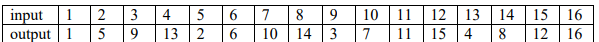
\includegraphics[scale=1]{Các công cụ và kĩ thuật sử dụng trong tấn công/S-boz.png}
    
\end{figure} 
Ta có bảng thống kê tương ứng với một số sai phân đầu vào:
\begin{figure}[H]
    \centering
    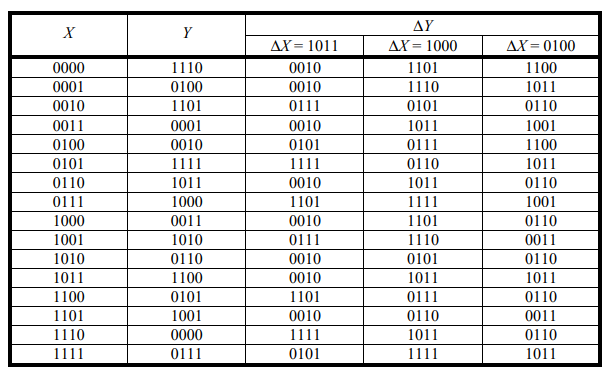
\includegraphics[scale=0.9]{Các công cụ và kĩ thuật sử dụng trong tấn công/sample diff sbox.png}
    
    \caption{Bảng thống kê tương ứng với một số sai phân đầu vào}
\end{figure}
Từ bảng trên, ta có thể thấy số lần xuất hiện của $\Delta Y = 0010$ với $\Delta X = 1011$ là 8 trên 16 giá trị có thể (tức là xác suất $\frac{8}{16}$); số lần xuất hiện của $\Delta Y = 1011$ với $\Delta X = 1000$ là 4 trên 16; số lần xuất hiện của $\Delta Y = 1010$ với $\Delta X =0100$ là 0 trên 16. 

Ta có thể tổng hợp thông tin hoàn thiện về tính chất Vi phân của 1 S-box dưới dạng một bảng Phân phối Sai phân với các hàng biểu diễn $\Delta X$ và các cột biểu diễn $\Delta Y$ (dưới dạng thập lục phân). Bảng Phân phối Sai phân của S-box đề cập ở trên được cho bởi bảng dưới đây. Mỗi phần tử trong bảng biểu diễn số lần xuất hiện của cặp sai phân $(\Delta X, \Delta Y)$ tương ứng. 
\begin{figure}[H]
    \centering
    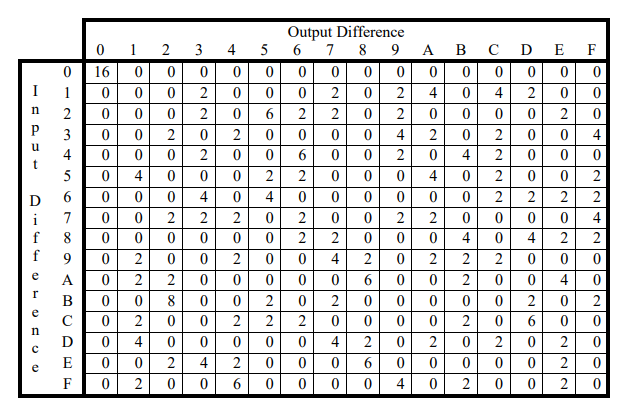
\includegraphics[scale=0.9]{Các công cụ và kĩ thuật sử dụng trong tấn công/diff distribution table.png}
    
    \caption{Bảng Phân phối Sai phân của S-box}
\end{figure}
\subsubsection{Phân tích Tính chất Vi phân của hệ mã hoàn chỉnh}
Ta sẽ sử dụng kiến trúc SPN (Substitution-Permutation Network) để mô phỏng việc Phân tích tính chất Vi phân này. Kiến trúc này được đề xuất bởi Feistel vào những năm 1973 và các toán tử cơ bản của nó tương tự với những gì tìm thấy ở DES hay rất nhiều hệ mã hiện đại khác, bao gồm cả Rijndael.

\begin{figure}[H]
    \centering
    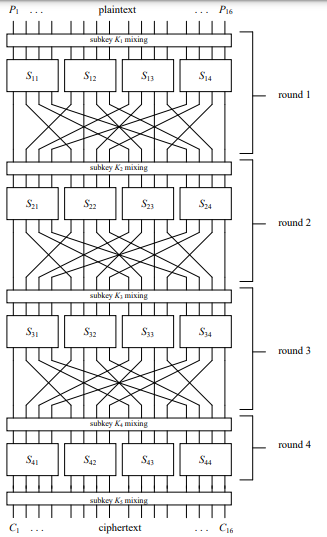
\includegraphics[scale=1.2]{Ảnh/triều/SPN.png}
    
    \caption{Kiến trúc SPN}
\end{figure}


Khi thông tin về tính chất Vi phân của các S-boxes trong SPN đã được tìm thấy, chúng ta có thể xác định tính chất Vi phân hữu dụng cho cả hệ. Điều này có thể thực hiện bằng cách ghép liên tiếp các cặp sai phân thích hợp. 

Xét tính chất Vi phân bao gồm $S_{12}, S_{23}, S_{32}, S_{33}.$ Đồ thị dưới đây biểu diễn ảnh hưởng của các cặp sai phân khi chúng di chuyển trên mạng, 
lưu ý tiến trình này xác định tính chất Vi phân của 3 vòng đầu tiên của hệ mã, không phải cả 4 vòng. Chúng ta sẽ thấy việc này hữu ích cho việc khôi phục bit từ khóa phụ cuối cùng ở phần sau. 
\begin{figure}[H]
    \centering
    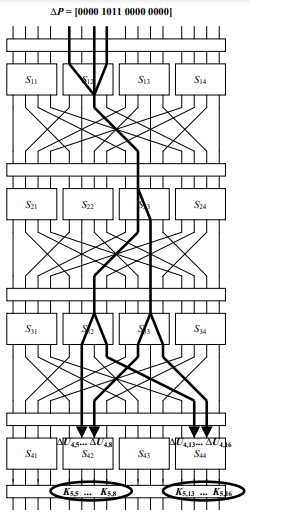
\includegraphics[scale=0.9]{Các công cụ và kĩ thuật sử dụng trong tấn công/spn1.png}
    
    \caption{Sample Differential Characteristics}
\end{figure}

Ta sử dụng cặp sai phân sau đây:

$S_{12}: \Delta X = B -> \Delta Y = 2$ với xác suất 8/16,

$S_{23}: \Delta X = 4 -> \Delta Y = 6$ với xác suất 6/16,

$S_{32}: \Delta X = 2 -> \Delta Y = 5$ với xác suất 6/16,

$S_{33}: \Delta X = 2 -> \Delta Y = 5$ với xác suất 6/16.

Sai phân đầu vào của hệ mã tương ứng với sai phân đầu vào tại vòng thứ nhất, được cho bởi:
$$ \Delta P = \Delta U_1 = [0000 1011 0000 0000]$$
Hệ quả là
$$ \Delta V_1 = [0000 0010 0000 0000]$$
và dựa vào cặp sai phân của $S_{12}$ ở trên và hoán vị ở vòng 1:
$$ \Delta U_2 = [0000 0000 0100 0000]$$ 
với xác suất 8/16 = 1/2 đối với sai phân đầu vào $\Delta P$. 

Tiếp theo vòng thứ 2, sử dụng cặp sai phân của $S_{23}$ ta có:
$$ \Delta V_2 = [0000 0000 0110 0000]$$
và hàm hoán vị ở vòng 2 cho ta:
$$ \Delta U_3 = [0000 0010 0010 0000]$$
với xác suất 6/16 đối với $\Delta U_2$ và xác suất 8/16 $\times$ 6/16 = 3/16 đối với $\Delta P$. 

Tương tự, ta sử dụng sai phân của S-box ở vòng thứ 3, $S_{23}$ và $S_{33}$, và hàm hoán vị ở vòng thứ 3 để thu được:
$$ \Delta V_3 = [0000 0101 0101 0000]$$ 
và 
$$ \Delta U_4 = [0000 0110 0000 0110]$$
với xác suất $(6/16)^2$ đối với $\Delta U_3$ và, do vậy, xác suất 8/16 $\times$ 6/16 $\times$ $(6/16)^2 = 27/1024$ đối với $\Delta P$.
\subsubsection{Trích xuất bit của khóa}
Một khi tính chất Vi phân của $R-1$ vòng của hệ mã $R$ vòng được khám phá với xác suất cao thích hợp, ta có thể tấn công hệ mã bằng cách khôi phục bit từ khóa phụ cuối cùng mà trong ví dụ của chúng ta, chính là việc khôi phục bit từ khóa phụ $K_5$. 

Quá trình mã hóa 1 phần được thực hiện với từng cặp bản rõ tương ứng với sai phân đầu vào $\Delta P$ cho tất cả các giá trị có thể của bộ phận khóa mục tiêu để đếm số lần trùng giữa sai phân đầu vào và sai phân đầu ra tương ứng.

Dưới đây là bảng mô phỏng tấn công bằng cách sinh 5000 bản rõ-mã chọn trước. Bộ phận khóa mục tiêu chính xác là $[K_{5,5}...K_{5,8}, K_{5,13}...K_{5,16}] = [0010,0100] = [2,4]_{hex}$. Như kỳ vọng, số lần trùng quan sát được lớn nhất là của bộ phận khóa $[2,4]_{hex},$ chứng tỏ cuộc tấn công đã thành công khôi phục bit của khóa phụ. Bảng dưới đây tổng hợp một phần dữ liệu từ việc phân tích các khóa phụ (Bảng hoàn thiện chứa 256 phần tử tương ứng 256 giá trị có thể của bộ phận khóa mục tiêu). Giá trị trong bảng thể hiện xấp xỉ xác suất xuất hiện của các cặp đúng đối với ứng viên khóa bộ phận.

\begin{figure}[H]
    \centering
    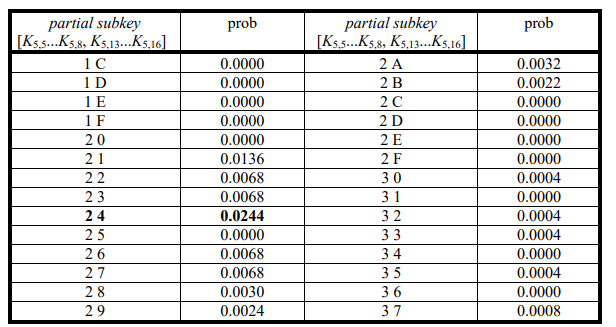
\includegraphics[scale=0.9]{Các công cụ và kĩ thuật sử dụng trong tấn công/experimential results diff.png}
    
    \caption{Kết quả Tấn công Vi phân thực nghiệm}
\end{figure}










\newpage
\subsection{Tấn công Tuyến tính (Linear Cryptanalysis) }
Các kết quả của phần này được trích từ \cite{hey2002}.
\subsubsection{Nguyên lý cơ bản}
Được đề xuất bởi Mitsuru Matsui trong cuốn "Advance in Cryptology" năm 1993, ông chứng minh Tấn công Tuyến tính có thể phá mã DES với $2^{47}$ bản rõ. Một năm sau, ông cải tiến kỹ thuật của mình và chứng minh chỉ cần $2^{43}$ bản rõ. Cho đến ngày nay, phương pháp tấn công Tuyến tính vẫn là phương pháp tấn công nhanh nhất để tấn công DES.

Tấn công Tuyến tính khai thác sự xuất hiện với xác suất cao của 1 biểu diễn tuyến tính nào đó giữa các bit của bản rõ và các bit của bản mã. Đây là dạng tấn công biết trước bản rõ, có nghĩa là kẻ tấn công được giả thiết có thông tin về 1 tập bản rõ và bản mã tương ứng nhất định. Trong nhiều ứng dụng và ngữ cảnh, có thể giả sử kẻ tấn công có thông tin về 1 tập ngẫu nhiên bản rõ và bản mã tương ứng.

Ý tưởng cơ bản của Tấn công tuyến tính là tìm kiếm một biểu diễn tuyến tính với xác suất đúng cao hơn ngẫu nhiên của các bit bản rõ, các bit bản mã, và các bit của khóa, cụ thể có dạng:
$$ X_{i_1} \oplus X_{i_2} \oplus ... \oplus X_{i_u} \oplus Y_{j_1} \oplus Y_{j_2} \oplus ... \oplus Y_{j_v} = K_{k_1} \oplus K_{k_2} \oplus ... \oplus K_{k_w} $$ 
hoặc dạng tương đương 
$$X_{i_1} \oplus X_{i_2} \oplus ... \oplus X_{i_u} \oplus Y_{j_1} \oplus Y_{j_2} \oplus ... \oplus Y_{j_v} = 0 $$
Trong đó $X_i$ là bit thứ $i$ của $X$, $Y_j$ là bit thứ $j$ của $Y$, $\oplus$ ký hiệu cho phép toán XOR.

Giả sử $p_L$ là xác suất biểu diễn trên đúng khi chọn ngẫu nhiên bản rõ và bản mã tương ứng, ta định nghĩa độ lệch (\emph{bias}) tương ứng là $p_L - 1/2.$ Độ lớn của \emph{bias} càng lớn, chứng tỏ độ ngẫu nhiên của hệ mật càng yếu, khả năng tấn công Tuyến tính với ít bản rõ cho trước càng cao.

Trước khi đi vào phân tích tính chất tuyến tính của 1 hệ mã cụ thể ta giới thiệu 1 công cụ hỗ trợ cho việc tính toán \emph{bias} một cách đơn giản hơn:

\textbf{(Piling-up Lemma)} Cho $n$ biến ngẫu nhiên độc lập toàn thể $X_1, X_2,..., X_n$. Khi đó:
    $$P(X_1 \oplus X_2 \oplus ... \oplus X_n = 0) = \frac{1}{2} + 2^{n-1} \prod_{i=1}^n \epsilon_i,  $$
    trong đó $\epsilon_i$ là độ lệch (\emph{bias}) của $X_i$.
\subsubsection{Phân tích tính chất Tuyến tính của S-box}
Ta vẫn sử dụng S-box giống như ở phần trước:
Ta sẽ phân tích tính chất Vi phân của S-box sau:
\begin{figure}[H]
    \centering
    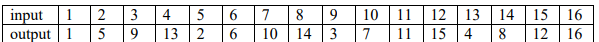
\includegraphics[scale=0.9]{Các công cụ và kĩ thuật sử dụng trong tấn công/S-boz.png}
\end{figure}
Ví dụ, xét biểu diễn tuyến tính $X_2 \oplus X_3 \oplus Y_1 \oplus Y_3 \oplus Y_4 = 0$ hay một cách tương đương $ X_2 \oplus  X_3 = Y_1 \oplus Y_3 \oplus Y_4.$ Kiểm tra tất cả 16 giá trị có thể của $X$ và đối chiếu với đầu ra tương ứng của $Y$, ta quan sát được biểu thức đúng với 12 trên 16 trường hợp. Như vậy giá trị \emph{bias} trong trường hợp này là $\frac{12}{16}-\frac{1}{2} = \frac{1}{4}.$ Tương tự ta có thể tính toán, với phương trình $X_1 \oplus X_4 = Y_2$ có giá trị \emph{bias} là 0 và phương trình $X_3 \oplus X_4 = Y_1 \oplus Y_4$ có độ \emph{bias} là $\frac{-3}{8}.$
Khả năng thành công của tấn công, như chúng ta sẽ thấy, phụ thuộc vào độ lớn của giá trị \emph{bias} này.

Ta có bảng phân tích một số biểu diễn xấp xỉ tuyến tính  của S-box:
 \begin{figure}
    \centering
    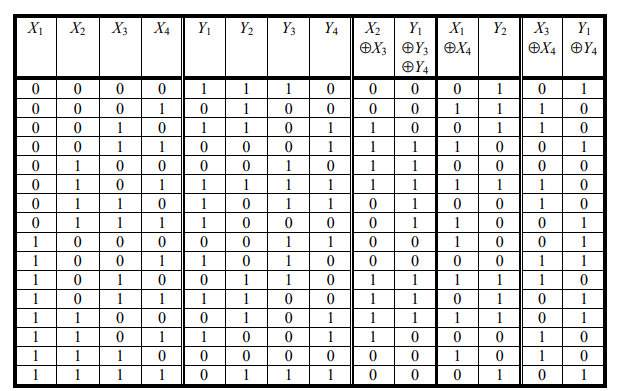
\includegraphics[scale = 0.9]{Các công cụ và kĩ thuật sử dụng trong tấn công/sample linear sbox.png}
    \caption{Phân tích một số biểu diễn xấp xỉ tuyến tính S-box}
    
    \end{figure}

    Kết quả tính toán cụ thể tất cả các xấp xỉ tuyến tính của S-box có thể cho bởi bảng Xấp xỉ Tuyến tính dưới đây. Mỗi phần tử trong bảng biểu diễn số lần trùng nhau giữa giá trị của phương trình tuyến tính của tổng các bit đầu vào và phương trình tuyến tính tổng các bit đầu ra (dưới dạng thập lục phân) trừ đi 8. Ví dụ, \emph{bias} của phương trình $X_3 \oplus X_4 = Y_1 \oplus Y_4$ (tương ứng với đầu vào hệ thập lục phân 3 và đầu ra 9) là $\frac{-6}{16} = \frac{-3}{8}$ và xác suất phương trình nhận giá trị đúng là $\frac{1}{2} - \frac{3}{8} = \frac{1}{8}$.
    \begin{figure}
    \centering
    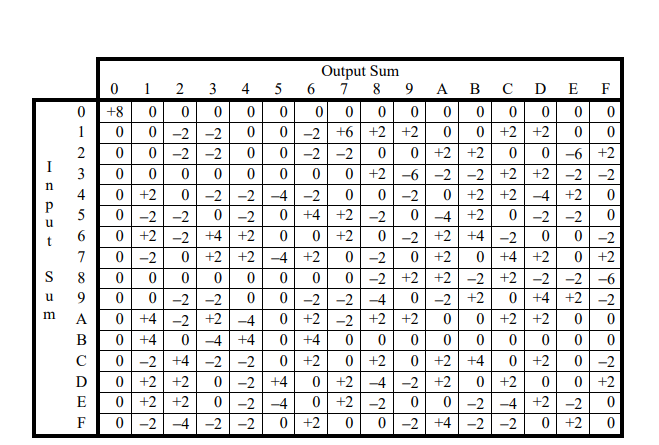
\includegraphics[scale = 0.9]{Các công cụ và kĩ thuật sử dụng trong tấn công/linear approx table.png}
    \caption{Bảng xấp xỉ tuyến tính S-box}
    
    \end{figure}
\subsubsection{Phân tích tính chất Tuyến tính của hệ mã hoàn chỉnh}
Tương tự như phần về Tấn công Vi phân, khi đã có thông tin về xấp xỉ tuyến tính của tất cả S-box trong SPN, chúng ta có thể xác định xấp xỉ tuyến tính cho cả hệ mã. Điều này có thể thực hiện bằng cách ghép liên tiếp các xấp xỉ tuyến tính thích hợp. Ta sẽ đưa ra ví dụ dưới đây:

Xét xấp xỉ tuyến tính bao gồm $S_{12}, S_{22}, S_{32}, S_{34}$ như hình dưới. Lưu ý rằng quá trình này đưa ra 1 biểu diễn xấp xỉ cho 3 vòng đầu của hệ mã chứ không phải cả 4 vòng. Ta sẽ thấy ở phần sau từ điều này có thể khôi phục lại 1 phần bit của khóa phụ cuối cùng.

\begin{figure}
    \centering
    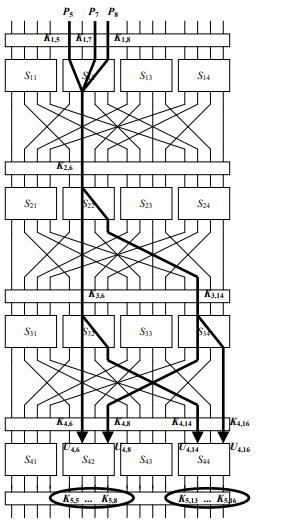
\includegraphics[scale = 1.5]{Các công cụ và kĩ thuật sử dụng trong tấn công/sample linear app.png}
    
    \caption{Sample Linear Approximation}
    \end{figure}

Ta xét các xấp xỉ sau của S-box:
$$S_{12}: X_1 \oplus X_3 \oplus X_4 = Y_2$$ với xác suất 12/16 và bias +1/4,
$$ S_{22}: X_2 = Y_2 \oplus Y_4$$ với xác suất 4/16 và bias -1/4,
$$ S_{32}: X_2 = Y_2 \oplus Y_4$$ với xác suất 4/16 và bias -1/4, 
$$ S_{34} = X_2 \oplus Y_4$$ với xác suất 4/16 và bias -1/4.

Gọi $U_i(V_i)$ thể hiện khối 16 bit đầu vào (đầu ra) tại vòng thứ $i$ của S-box và $U_{i,j} (V_{i,j})$ thể hiện bit thứ $j$ của khối $U_i (V_i)$. Tương tự, gọi $K_i$ là khối khóa phụ tại vòng thứ $i$.

Ta có  $U_1 = P \oplus K_1$, sử dụng xấp xỉ tuyến tính ở vòng thứ nhất, ta có:
$$ V_{1,6} = U_{1,5} \oplus U_{1,7} \oplus U_{1,8} = (P_5 \oplus K_{1,5}) \oplus (P_7 \oplus K_{1,7}) \oplus (P_8 \oplus K_{1,8})$$
với xác suất 3/4. Với xấp xỉ ở vòng thứ 2, ta có:
$$ V_{2,6} \oplus V_{2,8} = U_{2,6}$$
với xác suất 1/4. Từ $U_{2,6} = V_{1,6} \oplus K_{2,6}$, ta thu được xấp xỉ dưới dạng 
$$ V_{2,6} \oplus V_{2,8} = V_{1,6} \oplus K_{2,6}$$ với xác suất 1/4 và từ đó ta có :
$$ V_{2,6} \oplus V_{2,8} \oplus P_5 \oplus P_7 \oplus P_8 \oplus K_{1,5} \oplus K_{1,7} \oplus K_{1,8} \oplus K_{2,6} = 0$$
với xác suất 1/2 + 2(3/4-1/2)(1/4-1/2) = 3/8 theo Bổ đề Pilling Up.

Ở vòng 3, ta có 
$$ V_{3,6} \oplus V_{3,8} = U_{3,6}  $$ 
với xác suất 1/4 và 
$$ V_{3,14} \oplus V_{3,16} = U_{3,14}$$
với xác suất 1/4. Do đó, từ $U_{3,6} = V_{2,6} \oplus K_{3,6}$ và $U_{3,14} = V_{2,8} \oplus K_{3,14}$ ta có:
$$V_{3,6} \oplus V_{3,8} \oplus V_{3,14} \oplus V_{3,16} \oplus V_{2,6} \oplus K_{3,6} \oplus V_{2,8} \oplus K_{3,14} = 0$$
với xác suất $1/2 + 2(1/4-1/2)^2 = 5/8$.

Từ đó ta có:
$$ V_{3,6} \oplus V_{3,8} \oplus V_{3,14} \oplus V_{3,16} \oplus P_5 \oplus P_7 \oplus P_8 \oplus K_{1,5} \oplus K_{1,7} \oplus K_{1,8} \oplus K_{2,6} \oplus K_{3,6} \oplus K_{3,14} = 0.$$

Chú ý rằng $U_{4,6} = V_{3,6} \oplus K_{4,6}$, $U_{4,8} = V_{3,14} \oplus K_{4,8},$ $U_{4,14} = V_{3,8} \oplus K_{4,14}$ và $U_{4,16} = V_{3,16} \oplus K_{4,16},$ ta có thể viết lại như sau: 
$$ U_{4,6} \oplus U_{4,8} \oplus U_{4,14} \oplus U_{4,16} \oplus P_5 \oplus P_7 \oplus P_8 \oplus \small{\sum_{K}} = 0$$ \\
với
$\sum_{K} = K_{1,5} \oplus K_{1,7} \oplus K_{1,8} \oplus K_{2,6} \oplus K_{3,6} \oplus K_{3,14} \oplus K_{4,6} \oplus K_{4,8} \oplus K_{4,14} \oplus K_{4,16}$
và $\sum_K$ cố định bằng 0 hoặc 1 tùy vào khóa của hệ mã. Theo bổ đề Pilling Up, biểu thức trên đúng với xác suất 15/32 (và bias -1/32).
Như vậy biểu thức
 $$ U_{4,6} \oplus U_{4,8} \oplus U_{4,14} \oplus U_{4,16} \oplus P_5 \oplus P_7 \oplus P_8 = 0$$ 
 đúng với xác suất 15/32 hoặc 17/32. Nói cách khác, ta có 1 xấp xỉ tuyến tính cho 3 vòng đầu của cipher với độ lớn bias 1/32. Phần tiếp theo ta sử dụng điều này để khôi phục bit từ khóa.
 \subsubsection{Khôi phục bit từ khóa}
Giống như phần Tấn công Tuyến tính, ta có thể trích ra 1 phần bit của khóa $K_5$ sau 3 vòng Xấp xỉ tuyến tính. Quy trình bao gồm với mọi giá trị có thể của khóa bộ phận mục tiêu, bit của bản mã tương ứng được XOR với bit của khóa bộ phận mục tiêu và kết quả được chạy ngược lại qua S-box tương ứng. Điều này được thực hiện với tất cả cặp bản rõ, bản mã đã biết và 1 biến đếm được sử dụng với mỗi khóa bộ phận mục tiêu. Biến đếm này tăng mỗi lần biểu diễn tuyến tính đúng với bit ở vòng cuối của S-box và bản rõ đã biết. Khóa bộ phận mục tiêu có biến đếm lệch lớn nhất so với 1 nửa độ lớn không gian bản rõ - bản mã được cho là khóa bộ phận chính xác.

Dưới đây là bảng mô phỏng tấn công với 10000 bản rõ - bản mã biết trước đối với 2 khóa bộ phận mục tiêu $[K_{5,5}...K_{5,8}] = [0010]$ (hex 2) và $[K_{5,13}...K_{5,16} = [0100]$ (hex 4). Như đã dự đoán, $[2,4]_{hex}$ có biến đếm lệch nhiều nhất so với 5000, và trong thực tế, cũng là khóa bộ phận thực sự của khóa gốc ban đầu.
    \begin{figure}
    \centering
    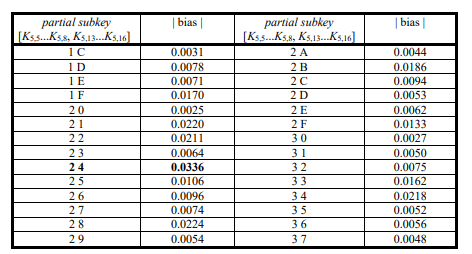
\includegraphics[scale = 0.9]{Các công cụ và kĩ thuật sử dụng trong tấn công/exp linear.png}
    
    \caption{Kết quả thực nghiệm Tấn công Tuyến tính}
    \end{figure}
    